% The 8th Joint Workshop on Machine Perception and Robotics
% --MPR 2012 Fukaoka, Japan, Oct. 16-17, 2012

% This file is edited based on the formatting of IEEE Conference Proceedings

% Edit it to your own paper. You can modify this file and MPR-head.tex

%% This file contains instructions on preparing your own paper for IEEE conference
%% but you can also use it as a LaTeX template for your own paper.
%% Some of the settings (mainly margins) are changed.
%% only A4 paper is allowed, 10pt normal size text and we use conference
%% option of the IEEEtran style file.
%% IEEEtran.cls (at least 2005/09/13 version V1.6c) can be downloaded from IEEE
%% Make sure that it is located in a path that LaTeX can find it.
%% The pdf file is produced by using pdflatex command.
%% If you want to use dvi -> ps -> pdf then you will need
%% to add/change the packages and use eps figures.
%%
\documentclass[conference,10pt,a4paper]{IEEEtran}
%\usepackage[pdftex]{graphicx}
\usepackage{graphicx}
\usepackage{diagbox}
\usepackage[colorlinks,linkcolor=blue]{hyperref}

\addtolength {\topmargin}{-1truemm}
\textwidth 184truemm
\textheight 235truemm
\columnsep 4truemm
%
\evensidemargin -11truemm
\oddsidemargin -11truemm

%% bare_conf.tex 
%% V1.2
%% 2002/11/18
%% by Michael Shell
%% mshell@ece.gatech.edu
%% 
%% NOTE: This text file uses MS Windows line feed conventions. When (human)
%% reading this file on other platforms, you may have to use a text
%% editor that can handle lines terminated by the MS Windows line feed
%% characters (0x0D 0x0A).
%% 
%% This is a skeleton file demonstrating the use of IEEEtran.cls 
%% (requires IEEEtran.cls version 1.6b or later) with an IEEE conference paper.
%% 
%% Support sites:
%% http://www.ieee.org
%% and/or
%% http://www.ctan.org/tex-archive/macros/latex/contrib/supported/IEEEtran/ 
%%
%% This code is offered as-is - no warranty - user assumes all risk.
%% Free to use, distribute and modify.

% *** Authors should verify (and, if needed, correct) their LaTeX system  ***
% *** with the testflow diagnostic prior to trusting their LaTeX platform ***
% *** with production work. IEEE's font choices can trigger bugs that do  ***
% *** not appear when using other class files.                            ***
% Testflow can be obtained at:
% http://www.ctan.org/tex-archive/macros/latex/contrib/supported/IEEEtran/testflow


% Also note that the "draftcls" or "draftclsnofoot", not "draft", option
% should be used if it is desired that the figures are to be displayed in
% draft mode.


% some very useful LaTeX packages include:

%\usepackage{cite}      % Written by Donald Arseneau
                        % V1.6 and later of IEEEtran pre-defines the format
                        % of the cite.sty package \cite{} output to follow
                        % that of IEEE. Loading the cite package will
                        % result in citation numbers being automatically
                        % sorted and properly "ranged". i.e.,
                        % [1], [9], [2], [7], [5], [6]
                        % (without using cite.sty)
                        % will become:
                        % [1], [2], [5]--[7], [9] (using cite.sty)
                        % cite.sty's \cite will automatically add leading
                        % space, if needed. Use cite.sty's noadjust option
                        % (cite.sty V3.8 and later) if you want to turn this
                        % off. cite.sty is already installed on most LaTeX
                        % systems. The latest version can be obtained at:
                        % http://www.ctan.org/tex-archive/macros/latex/contrib/supported/cite/

%\usepackage{graphicx}  % Written by David Carlisle and Sebastian Rahtz
                        % Required if you want graphics, photos, etc.
                        % graphicx.sty is already installed on most LaTeX
                        % systems. The latest version and documentation can
                        % be obtained at:
                        % http://www.ctan.org/tex-archive/macros/latex/required/graphics/
                        % Another good source of documentation is "Using
                        % Imported Graphics in LaTeX2e" by Keith Reckdahl
                        % which can be found as esplatex.ps and epslatex.pdf
                        % at: http://www.ctan.org/tex-archive/info/

% However, be warned that pdflatex will require graphics to be in PDF
% (not EPS) format and will preclude the use of PostScript based LaTeX
% packages such as psfrag.sty and pstricks.sty. IEEE conferences typically
% allow PDF graphics (and hence pdfLaTeX). However, IEEE journals do not
% (yet) allow image formats other than EPS or TIFF. Therefore, authors of
% journal papers should use traditional LaTeX with EPS graphics.
%
% The path(s) to the graphics files can also be declared: e.g.,
%\graphicspath{{../figures/}}
% if the graphics files are not located in the same directory as the
% .tex file. This can be done in each branch of the conditional above
% (after graphicx is loaded) to handle the EPS and PDF cases separately.
% In this way, full path information will not have to be specified in
% each \includegraphics command.
%
% Note that, when switching from latex to pdflatex and vice-versa, the new
% compiler will have to be run twice to clear some warnings.


%\usepackage{psfrag}    % Written by Craig Barratt, Michael C. Grant,
                        % and David Carlisle
                        % This package allows you to substitute LaTeX
                        % commands for text in imported EPS graphic files.
                        % In this way, LaTeX symbols can be placed into
                        % graphics that have been generated by other
                        % applications. You must use latex->dvips->ps2pdf
                        % workflow (not direct pdf output from pdflatex) if
                        % you wish to use this capability because it works
                        % via some PostScript tricks. Alternatively, the
                        % graphics could be processed as separate files via
                        % psfrag and dvips, then converted to PDF for
                        % inclusion in the main file which uses pdflatex.
                        % Docs are in "The PSfrag System" by Michael C. Grant
                        % and David Carlisle. There is also some information 
                        % about using psfrag in "Using Imported Graphics in
                        % LaTeX2e" by Keith Reckdahl which documents the
                        % graphicx package (see above). The psfrag package
                        % and documentation can be obtained at:
                        % http://www.ctan.org/tex-archive/macros/latex/contrib/supported/psfrag/

\usepackage{subfigure} % Written by Steven Douglas Cochran
                        % This package makes it easy to put subfigures
                        % in your figures. i.e., "figure 1a and 1b"
                        % Docs are in "Using Imported Graphics in LaTeX2e"
                        % by Keith Reckdahl which also documents the graphicx
                        % package (see above). subfigure.sty is already
                        % installed on most LaTeX systems. The latest version
                        % and documentation can be obtained at:
                        % http://www.ctan.org/tex-archive/macros/latex/contrib/supported/subfigure/

\usepackage{url}       % Written by Donald Arseneau
                        % Provides better support for handling and breaking
                        % URLs. url.sty is already installed on most LaTeX
                        % systems. The latest version can be obtained at:
                        % http://www.ctan.org/tex-archive/macros/latex/contrib/other/misc/
                        % Read the url.sty source comments for usage information.

%\usepackage{stfloats}  % Written by Sigitas Tolusis
                        % Gives LaTeX2e the ability to do double column
                        % floats at the bottom of the page as well as the top.
                        % (e.g., "\begin{figure*}[!b]" is not normally
                        % possible in LaTeX2e). This is an invasive package
                        % which rewrites many portions of the LaTeX2e output
                        % routines. It may not work with other packages that
                        % modify the LaTeX2e output routine and/or with other
                        % versions of LaTeX. The latest version and
                        % documentation can be obtained at:
                        % http://www.ctan.org/tex-archive/macros/latex/contrib/supported/sttools/
                        % Documentation is contained in the stfloats.sty
                        % comments as well as in the presfull.pdf file.
                        % Do not use the stfloats baselinefloat ability as
                        % IEEE does not allow \baselineskip to stretch.
                        % Authors submitting work to the IEEE should note
                        % that IEEE rarely uses double column equations and
                        % that authors should try to avoid such use.
                        % Do not be tempted to use the cuted.sty or
                        % midfloat.sty package (by the same author) as IEEE
                        % does not format its papers in such ways.

\usepackage{amsmath}   % From the American Mathematical Society
                        % A popular package that provides many helpful commands
                        % for dealing with mathematics. Note that the AMSmath
                        % package sets \interdisplaylinepenalty to 10000 thus
                        % preventing page breaks from occurring within multiline
                        % equations. Use:
\interdisplaylinepenalty=2500
                        % after loading amsmath to restore such page breaks
                        % as IEEEtran.cls normally does. amsmath.sty is already
                        % installed on most LaTeX systems. The latest version
                        % and documentation can be obtained at:
                        % http://www.ctan.org/tex-archive/macros/latex/required/amslatex/math/



% Other popular packages for formatting tables and equations include:

\usepackage{array}
% Frank Mittelbach's and David Carlisle's array.sty which improves the
% LaTeX2e array and tabular environments to provide better appearances and
% additional user controls. array.sty is already installed on most systems.
% The latest version and documentation can be obtained at:
% http://www.ctan.org/tex-archive/macros/latex/required/tools/

% Mark Wooding's extremely powerful MDW tools, especially mdwmath.sty and
% mdwtab.sty which are used to format equations and tables, respectively.
% The MDWtools set is already installed on most LaTeX systems. The lastest
% version and documentation is available at:
% http://www.ctan.org/tex-archive/macros/latex/contrib/supported/mdwtools/


% V1.6 of IEEEtran contains the IEEEeqnarray family of commands that can
% be used to generate multiline equations as well as matrices, tables, etc.


% Also of notable interest:

% Scott Pakin's eqparbox package for creating (automatically sized) equal
% width boxes. Available:
% http://www.ctan.org/tex-archive/macros/latex/contrib/supported/eqparbox/



% Notes on hyperref:
% IEEEtran.cls attempts to be compliant with the hyperref package, written
% by Heiko Oberdiek and Sebastian Rahtz, which provides hyperlinks within
% a document as well as an index for PDF files (produced via pdflatex).
% However, it is a tad difficult to properly interface LaTeX classes and
% packages with this (necessarily) complex and invasive package. It is
% recommended that hyperref not be used for work that is to be submitted
% to the IEEE. Users who wish to use hyperref *must* ensure that their
% hyperref version is 6.72u or later *and* IEEEtran.cls is version 1.6b 
% or later. The latest version of hyperref can be obtained at:
%
% http://www.ctan.org/tex-archive/macros/latex/contrib/supported/hyperref/
%
% Also, be aware that cite.sty (as of version 3.9, 11/2001) and hyperref.sty
% (as of version 6.72t, 2002/07/25) do not work optimally together.
% To mediate the differences between these two packages, IEEEtran.cls, as
% of v1.6b, predefines a command that fools hyperref into thinking that
% the natbib package is being used - causing it not to modify the existing
% citation commands, and allowing cite.sty to operate as normal. However,
% as a result, citation numbers will not be hyperlinked. Another side effect
% of this approach is that the natbib.sty package will not properly load
% under IEEEtran.cls. However, current versions of natbib are not capable
% of compressing and sorting citation numbers in IEEE's style - so this
% should not be an issue. If, for some strange reason, the user wants to
% load natbib.sty under IEEEtran.cls, the following code must be placed
% before natbib.sty can be loaded:
%
% \makeatletter
% \let\NAT@parse\undefined
% \makeatother
%
% Hyperref should be loaded differently depending on whether pdflatex
% or traditional latex is being used:
%
%\ifx\pdfoutput\undefined
%\usepackage[hypertex]{hyperref}
%\else
%\usepackage[pdftex,hypertexnames=false]{hyperref}
%\fi
%
% Pdflatex produces superior hyperref results and is the recommended
% compiler for such use.



% *** Do not adjust lengths that control margins, column widths, etc. ***
% *** Do not use packages that alter fonts (such as pslatex).         ***
% There should be no need to do such things with IEEEtran.cls V1.6 and later.


% correct bad hyphenation here
\hyphenation{op-tical net-works semi-conduc-tor IEEEtran}



\begin{document}

% paper title
\title{Semantic Segmentation of 3D LiDAR Data at Dynamic Urban Scenes}


% avoiding spaces at the end of the author lines is not a problem with
% conference papers because we don't use \thanks or \IEEEmembership


\author{\authorblockN
	{Biao Gao\authorrefmark{1},
		Jilin Mei\authorrefmark{1}, 
		Donghao Xu\authorrefmark{1},
		Xijun Zhao\authorrefmark{2},
		Wen Yao\authorrefmark{2},
		Huijing Zhao\authorrefmark{1}}
\authorblockA{\authorrefmark{1}Peking University, Beijing, China}
\authorblockA{\authorrefmark{2}201 Institution, Beijing, China}}


% use only for invited papers
%\specialpapernotice{(Invited Paper)}

% make the title area
\maketitle

\begin{abstract}
This work studies semantic segmentation of 3D LiDAR data at dynamic urban scenes. LiDAR data plays an important role of perception in autonomous driving system. However, most semantic segmentation methods and datasets are designed for camera data nowadays. In this work, we propose a method which can generate semantic segmentation of LiDAR data and we evaluate its performance on a new 3D point cloud dataset collected in dynamic urban scenes by our driving platform. The experiments show that our method can recognize more kinds of labels and achieve an impressive result in dynamic urban scenes.
\end{abstract}

% no key words

\section{Introduction}
% no \PARstart
empty

\section{Related works}
% no \PARstart
empty

\section{Methodology}

\subsection{Data Preprocessing}
The point cloud data for LiDAR is sparse and unorganized, so it is time-consuming to find neighboring relations between different points. In order to process these unorganized point cloud data with deep convolutional neural network, we convert the point cloud data into 2D range image by cylindrical projection. After that, it will be easier to implement deep convolution neural network on the LiDAR data.

After cylindrical projection, the point cloud data will be encoded as a dense matrix with shape of $[H,W,C]$. $H$ means the number of lines for the specific LiDAR sensor (such as $H=32$ for Velodyne HDL-32E). $W$ equals to the number of points within each LiDAR scan line. $C$ is the channels' number in the range image. Here, $C$ is set to 3, which represents $[Range,Intensity,Height]$ three channels.

For each point $p_k=\langle x_k,y_k,z_k\rangle$ from the raw point cloud set $P$, the value of $Range$ in range image $R$ is defined as $r_k$:
 
\begin{equation}
r_k=\sqrt{{x_k}^2+{y_k}^2+{z_k}^2},  r_k\subset [0,255]	
\end{equation} 

Similarly, the values of $Intensity$ and $Height$ are normalized into $[0,255]$. These channels are very important properties of LiDAR data, which are enough to describe various objects in dynamic urban scenes.
 
\subsection{Problem Definition}

Let $X$ denotes the range image extracted by cylindrical projection of 3D point cloud data $S$. In this kind of projection, there is a one-to-one correspondence between a 3D point in one frame point cloud data and a pixel in the range image $X$. As a result, the semantic segmentation task of 3D point cloud data is equal with giving each pixel $x$ in the range image $X$ a label $y$. The problem of this work is formulated as learning a semantic segmentation model $f_{\theta}$ which maps each pixel $x$ to a label $y\in\{1,...,K\}$, and subsequently associate $y$ to the 3D points of $S$.

\begin{equation}
f_{\theta}: x\to y \in \{1,...,K\}
\end{equation}

The data samples are in the form of range images $X$. Given a set of supervised data samples $X_l=\{x_i, y_i\}$, where $\{x_i\}$ traverses each pixel of $X$ and $\{y_i\}$ are labels for $\{x_i\}$, annotated manually by human annotators. 
In order to learning a semantic segmentation model $f_\theta$, we need to find the best parameter set $\theta^*$ that minimize a loss function $L$ as below.

\begin{equation}
\theta^{*}=\mathop{\arg\max}_{\theta}L(X_l; \theta)
\end{equation}

\subsection{Network Architecture and Loss Function}
We use a FCN (Fully Convolutional Network) architecture for this semantic segmentation task.
Compared with common deep convolutional networks, it removes last fully connected layers, and replaces them with the in-network up-sampled or de-convolutional predictions of convolutional layers as predicted feature maps. During training procedure, it generally computes cross-entropy like losses in pixel-wise, between the predicted labels and ground truths.

Our network is trained via end-to-end guided by the designed loss function. Because the number of pixels are imbalanced between different classes and a lot of invalid or unknown-class pixels, the following multi-class weighted cross entropy loss function is designed to regular the weights between imbalanced classes.

For labeled data $X_l$, we implement some changes on the widely-used definition of cross entropy, and define loss function $L_l$ as below:

\begin{equation}
\begin{split}
&\varGamma_{i,j}=\{
	\begin{array}{lr}
	\overrightarrow{\varphi_k} ,\quad\quad if \quad [y_{i,j}\neq k \quad and\quad y_{i,j}\neq0]	\\
	\overrightarrow{0} ,\quad\quad\quad\quad\quad\quad  otherwise
	\end{array}	\\
	\\
&\textit{}L_l(X_l,Y_l;\theta)=-\frac{1}{H*W}\sum_{i=0}^{H-1}\sum_{j=0}^{W-1}\sum_{k=0}^K{\varGamma_{i,j}\omega_{k}ln(P^k_{\theta}(x_{i,j}))}
\end{split}
\end{equation}
Where $\varGamma_{i,j}$ is a one-hot vector $\varphi_k$ of label $k$, if $y_{i,j}\neq k$ and $y_{i,j}\neq0$. Label 0 means invalid or unknown pixels, including many fine fragments belong to background or hard to be annotated, so we don't want to evaluate these pixels if they are predicted as non-zero labels. $\omega_{k}$ here is used to balance the sample numbers between different labels and $P^k_{\theta}(x_{i,j})$ is the probability that pixel $x_{i,j}$ be assigned a label $k$ by our semantic segmentation model with the set of parameters $\theta$.


\section{Experiment}
\subsection{Data Set}
The performance of the proposed method is evaluated on a dynamic campus data set collected by an instrumented vehicle, which has a GPS/IMU suite and a Velodyne-HDL32, as shown in Fig. \ref{fig:collect_route}. The total route contains 1375 LiDAR frames. 880 frames for training, 220 frames for validation and 275 frames for testing.

\begin{figure}[ht]
\centering
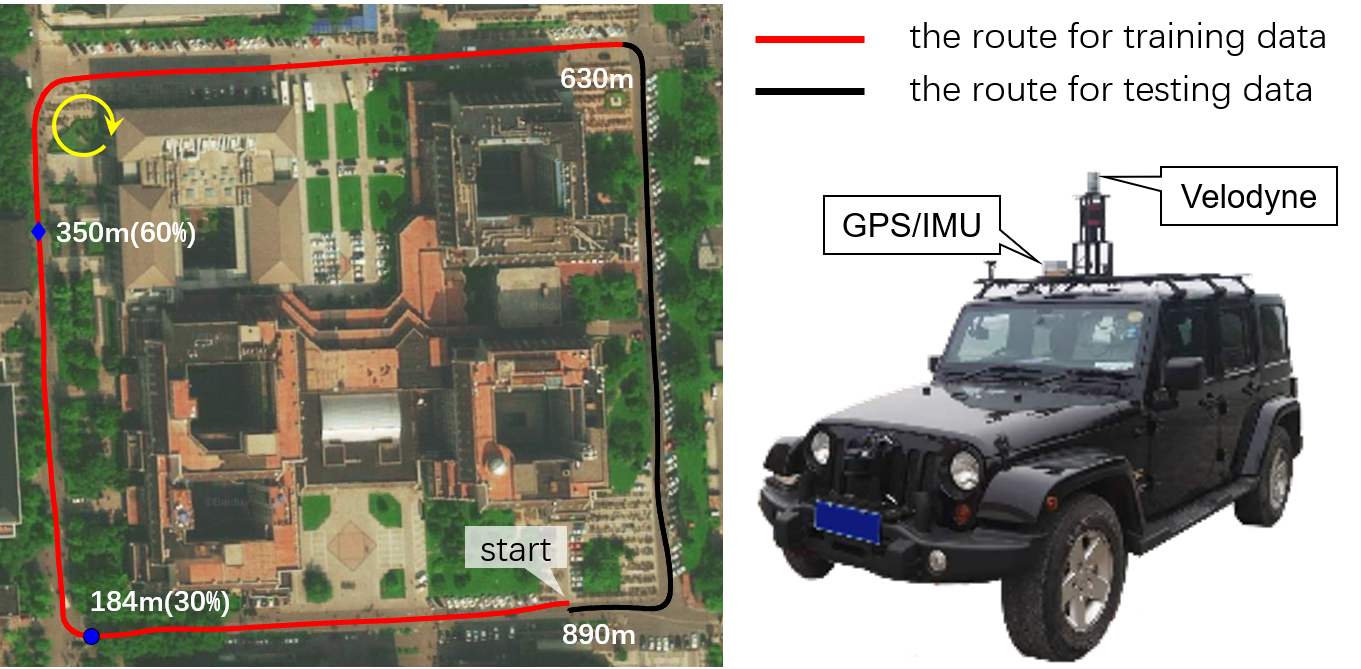
\includegraphics[width=1.0\linewidth]{fig/collect_route}
% 这个图要更新!!!!!!!!!
\caption{The routes of data collection and the platform configuration.}
\label{fig:collect_route}
\end{figure}

\begin{table}[hb]
	\begin{center} \caption{Categories Distribution in Dataset}
		\label{category_distribution}
		\renewcommand{\arraystretch}{1.3}
		\begin{tabular}{|c|c|c|c|c|c|}
			\hline
			 - & People & Car & Vegetation & Building & Road	\\
			\hline
			Pixels & 733,664 & 257,239 & 4,661,880 & 6,579,360 & 16,856,614	\\
			\hline
		\end{tabular}
	\end{center}
\end{table}

High quality pixel-level annotation is necessary for network training. Instead of working on the raw point cloud, human annotators work on the range image where object regions are associated with the ones in adjacent frames. Annotators only need to assign the category of some region in one frame, then a series of associated regions are marked with the same label. Although sometimes the data association brings errors, it largely reduce the annotation time. 

The categories distribution in this dataset is shown in TABLE . \ref{category_distribution}. Obviously, the data distribution is imbalanced between categories. So, we apply each label an unique weight based on data distribution to reduce the influence of data imbalance.

\subsection{Setup}
Our method is implemented with a FCN (Fully Convolutional Network). The range image size is 1080x32, which width is down-sampled for efficiency. A small batch size for training sets will be better. The network is implemented with TensorFlow in the environment with NVIDIA TITAN X GPU. We use the AdamOptimizer with 1e-5 learning rate.

It's important to aware that our data frames are captured sequentially. In order to avoid data correlation between adjacent frames, shuffling them before training process is necessary.

\subsection{Preparing your Electronic Paper}

{\em Type sizes and typefaces}: Follow the type sizes specified in
Table~\ref{table1}. As an aid in gauging type size, 1 point is
about 0.35~mm. The size of the lowercase letter ``j'' will give
the point size. Times New Roman is the preferred font.

{\em 1) US Letter Margins}:  top = 0.75 inches, bottom = 1 inch, side = 0.625 inches. 
Each column measures 3.5 inches wide, with a 0.25-inch measurement between columns.

{\em 2) A4 Margins}: top = 19mm, bottom = 43mm, side = 13 mm. The A4 column width is 
88mm (3.45 in). The space between the two columns is 4mm (0.17 in). Paragraph indentation 
is 3.5 mm (0.14 in).

\begin{table}[hb]
\begin{center} \caption{Type Sizes for Papers}
\label{table1}
\renewcommand{\arraystretch}{1.3}
\begin{tabular}{|c|p{34mm}|c|c|}
 \hline
Type & \multicolumn{3}{c|}{Appearance} \\
size &\multicolumn{3}{c|}{~} \\ \cline{2-4} (pts.) & Regular &
Bold & Italic \\ \hline
 6 & Table captions\footnotemark[1], table superscripts & & \\ \hline
 8 & Section titles\footnotemark[1], references, tables, table
 names\footnotemark[1],
 first letters in table captions\footnotemark[1], figure captions, footnotes,
 text subscripts, and superscripts &
& \\ \hline
 9 & & Abstract & \\ \hline
 10 & Authors' affiliations, main text, equations, first letters in
 section titles\footnotemark[1] & & Subheading \\ \hline
 11 & Authors' names & & \\ \hline
 24 & Paper title & & \\ \hline
\end{tabular}
\end{center}
\end{table}
\footnotetext[1]{Uppercase    ( {\bf It is recommended that footnotes be avoided. Instead, try to integrate the footnote information into the text.} )}

The column width is 82~mm (3.23 in). The space between the two columns is
6~mm (0.24 in). Paragraph indentation is 3.5 mm (0.14 in).

Left- and right-justify your columns. Use tables and figures to
adjust column length. On the last page of your paper, adjust the
lengths of the columns so that they are equal. Use automatic
hyphenation and check spelling.


\section{Helpful Hints}

\subsection{Figures and Tables - Subsection Example}

Position figures and tables at the tops and bottoms of columns. Avoid
placing them in the middle of columns. Large figures and tables may span
across both columns. Figure captions should be centered below the figures;
table captions should be centered above. Avoid placing figures and tables
before their first mention in the text. Use the abbreviation ``Fig. 1'',
even at the beginning of a sentence.

\subsubsection{Sub-subsection example}
Figure axis labels are often a source of confusion. Use words rather than
symbols. For example, write ``Magnetization'', or ``Magnetization, M'',
not just ``M.''  Put units in parentheses. Do not label axes only with
units. In the example, write ``Magnetization (A/m)'' or ``Magnetization (A
$\cdot$ m$^{-1}$).'' Do not label axes with a ratio of quantities and
units. For example, write ``Temperature (K)'', not ``Temperature/K.''

Multipliers can be especially confusing. Write ``Magnetization (kA/m)'' or
``Magnetization ($10^{3}$ A/m)''. Figure labels should be legible, about
10-point type.


\subsection{References}

Number citations consecutively in square brackets \cite{eason}.
Punctuation follows the bracket \cite{maxwell}. Refer simply to the
reference number, as in \cite{jacobs}. Use ``Ref. \cite{jacobs}'' or
``Reference \cite{jacobs}'' at the beginning of a sentence: ``Reference
\cite{jacobs} was the first ...''

Number footnotes separately in superscripts. Place the actual footnote at
the bottom of the column in which it was cited. Do not put footnotes in
the reference list. Use letters for table footnotes (see Table 1). IEEE
Transactions no longer use a journal prefix before the volume number. For
example, use ``IEEE Trans. Magn., vol. 25'', not ``vol. MAG-25''.

Give all authors' names; use ``et al.'' if there are six authors or more.
Papers that have not been published, even if they have been submitted for
publication, should be cited as "unpublished" \cite{elissa}. Papers that
have been accepted for publication should be cited as ``in press''
\cite{nicole}. In a paper title, capitalize the first word and all other
words except for conjunctions, prepositions less than seven letters, and
prepositional phrases.

\begin{figure}[t]
 \centering
% \includegraphics[scale=0.95] {fig1}
\caption{Magnetization as a function of applied field.} \label{figure1}
\end{figure}

For papers published in translated journals, first give the English
citation, then the original foreign-language citation \cite{yorozu}.


\subsection{Abbreviations and Acronyms}

Define abbreviations and acronyms the first time they are used in the
text, even after they have been defined in the abstract. Abbreviations
such as IEEE, SI, MKS, CGS, sc, dc, and rms do not have to be defined. Do
not use abbreviations in the title unless they are unavoidable.

\subsection{Equations}

Number equations consecutively with equation numbers in
parentheses flush with the right margin, as in (\ref{eq1}). To
make your equations more compact, you may use the solidus (/), the
exp function, or appropriate exponents. Italicize Roman symbols
for quantities and variables, but not Greek symbols. Use an en
dash (-) rather than a hyphen for a minus sign. Use parentheses to
avoid ambiguities in denominators. Punctuate equations with commas
or periods when they are part of a sentence, as in
\begin{equation}
 z = \sin^2 x + \cos^2 y.  \label{eq1}
\end{equation}
Symbols in your equation should be defined before the equation
appears or immediately following. Use ``(\ref{eq1}),'' not
``Eq.~(\ref{eq1})'' or ``equation~(\ref{eq1}),'' except at the
beginning of a sentence: ``Equation~(\ref{eq1}) is ...''


\subsection{Other Recommendations}

The Roman numerals used to number the section headings are
optional. If you do use them, do not number ACKNOWLEDGMENTS and
REFERENCES, and begin Subheadings with letters. Use two spaces
after periods (full stops). Hyphenate complex modifiers:
``zero-field-cooled magnetization.'' Avoid dangling participles,
such as, ``Using (\ref{eq1}), the potential was calculated.''
Write instead, ``The potential was calculated using (\ref{eq1}),''
or ``Using  (\ref{eq1}), we calculated the potential.''

Use a zero before decimal points: ``0.25'', not ``.25''. Use ``cm$^{3}$''
not ``cc''. Do not mix complete spellings and abbreviations of units:
``Wb/m$^{2}$'' or ``webers per square meter,'' not ``webers/m$^{2}$''.
Spell units when they appear in text: ``...a few henries'', not ``...a few
H.'' If your native language is not English, try to get a native
English-speaking colleague to proofread your paper. Do not add page
numbers.

\section{Units}

Use either SI (MKS) or CGS as primary units. (SI units are encouraged.)
English units may be used as secondary units (in parentheses). An
exception would be the use of English units as identifiers in trade, such
as ``3.5-inch disk drive.''

Avoid combining SI and CGS units, such as current in amperes and magnetic
field in oersteds. This often leads to confusion because equations do not
balance dimensionally.


\section{Some Common Mistakes}

The word ``data'' is plural, not singular. The subscript for the
permeability of vacuum is zero, not a lowercase letter ``o''. In American
English, periods and commas are within quotation marks, like ``this
period''. A parenthetical statement at the end of a sentence is punctuated
outside of the closing parenthesis (like this). (A parenthetical sentence
is punctuated within the parentheses.) A graph within a graph is an
``inset'', not an ``insert''. The word alternatively is preferred to the
word ``alternately'' (unless you mean something that alternates). Do not
use the word ``essentially'' to mean ``approximately'' or ``effectively.''
Be aware of the different meanings of the homophones  ``affect'' and
``effect,'' ``complement'' and ``compliment,'' ``discreet'' and
``discrete,'' ``principal'' and ``principle.'' Do not confuse ``imply''
and ``infer.'' The prefix ``non'' is not a word; it should be joined to
the word it modifies, usually without a hyphen. There is no period after
the ``et'' in the Latin abbreviation ``et al.'' The abbreviation ``i.e.''
means ``that is,'' and the abbreviation ``e.g.'' means ``for example.'' An
excellent style manual for science writers is \cite{young}.



% Reminder: the "draftcls" or "draftclsnofoot", not "draft", class option
% should be used if it is desired that the figures are to be displayed while
% in draft mode.

% An example of a floating figure using the graphicx package.
% Note that \label must occur AFTER (or within) \caption.
% For figures, \caption should occur after the \includegraphics.
%
%\begin{figure}
%\centering
%\includegraphics[width=2.5in]{myfigure}
% where an .eps filename suffix will be assumed under latex, 
% and a .pdf suffix will be assumed for pdflatex
%\caption{Simulation Results}
%\label{fig_sim}
%\end{figure}


% An example of a double column floating figure using two subfigures.
%(The subfigure.sty package must be loaded for this to work.)
% The subfigure \label commands are set within each subfigure command, the
% \label for the overall fgure must come after \caption.
% \hfil must be used as a separator to get equal spacing
%
%\begin{figure*}
%\centerline{\subfigure[Case I]{\includegraphics[width=2.5in]{subfigcase1}
% where an .eps filename suffix will be assumed under latex, 
% and a .pdf suffix will be assumed for pdflatex
%\label{fig_first_case}}
%\hfil
%\subfigure[Case II]{\includegraphics[width=2.5in]{subfigcase2}
% where an .eps filename suffix will be assumed under latex, 
% and a .pdf suffix will be assumed for pdflatex
%\label{fig_second_case}}}
%\caption{Simulation results}
%\label{fig_sim}
%\end{figure*}



% An example of a floating table. Note that, for IEEE style tables, the 
% \caption command should come BEFORE the table. Table text will default to
% \footnotesize as IEEE normally uses this smaller font for tables.
% The \label must come after \caption as always.
%
%\begin{table}
%% increase table row spacing, adjust to taste
%\renewcommand{\arraystretch}{1.3}
%\caption{An Example of a Table}
%\label{table_example}
%\begin{center}
%% Some packages, such as MDW tools, offer better commands for making tables
%% than the plain LaTeX2e tabular which is used here.
%\begin{tabular}{|c||c|}
%\hline
%One & Two\\
%\hline
%Three & Four\\
%\hline
%\end{tabular}
%\end{center}
%\end{table}


%\section{Conclusion}
%The conclusion goes here.

% conference papers do not normally have an appendix

% use section* for acknowledgement
\section*{Acknowledgment}
% optional entry into table of contents (if used)
%\addcontentsline{toc}{section}{Acknowledgment}

The preferred spelling of the word "acknowledgment" in America is without
an "e" after the "g". Try to avoid the stilted expression, "One of us
(R.B.G.) thanks ...". Instead, try "R.B.G. thanks ...". Put sponsor
acknowledgments in the unnumbered footnote on the first page.

% trigger a \newpage just before the given reference
% number - used to balance the columns on the last page
% adjust value as needed - may need to be readjusted if
% the document is modified later
%\IEEEtriggeratref{8}
% The "triggered" command can be changed if desired:
%\IEEEtriggercmd{\enlargethispage{-5in}}

% references section
% NOTE: BibTeX documentation can be easily obtained at:
% http://www.ctan.org/tex-archive/biblio/bibtex/contrib/doc/

% can use a bibliography generated by BibTeX as a .bbl file
% standard IEEE bibliography style from:
% http://www.ctan.org/tex-archive/macros/latex/contrib/supported/IEEEtran/testflow/bibtex
%\bibliographystyle{IEEEtran.bst}
% argument is your BibTeX string definitions and bibliography database(s)
%\bibliography{IEEEabrv,../bib/paper}
%
% <OR> manually copy in the resultant .bbl file
% set second argument of \begin to the number of references
% (used to reserve space for the reference number labels box)

\begin{thebibliography}{10}

\bibitem{eason} G. Eason, B. Noble, and I. N. Sneddon, ``On certain integrals of
Lipschitz-Hankel type involving products of Bessel functions,'' {\em Phil.
Trans. Roy. Soc. London}, vol. A247, pp. 529--551, April 1955.

\bibitem{maxwell} J. Clerk Maxwell, {\em A Treatise on Electricity and Magnetism}, 3rd ed.,
vol. 2. Oxford: Clarendon, 1892, pp.68--73.

\bibitem{jacobs} I. S. Jacobs and C. P. Bean, ``Fine particles, thin films and exchange
anisotropy,'' in {\em Magnetism}, vol. III, G. T. Rado and H. Suhl, Eds.
New York: Academic, 1963, pp. 271--350.

\bibitem{elissa} K. Elissa, ``Title of paper if known,'' unpublished.

\bibitem{nicole} R. Nicole, ``Title of paper with only first word capitalized'',
{\em J. Name Stand. Abbrev.}, in press.

\bibitem{yorozu} Y. Yorozu, M. Hirano, K. Oka, and Y. Tagawa, ``Electron spectroscopy
studies on magneto-optical media and plastic substrate interface,'' {\em
IEEE Transl. J. Magn. Japan}, vol. 2, pp. 740--741, August 1987 [Digests
9th Annual Conf. Magnetics Japan, p. 301, 1982].

\bibitem{young} M. Young, {\em The Technical Writer's Handbook}. Mill Valley, CA: University
Science, 1989.


\end{thebibliography}


% that's all folks
\end{document}
